% begin module polar-area-ex1
\begin{frame}
\begin{example}[Example 1, p. 686]
Find the area enclosed by one loop of the four-leaved rose \alert<handout:0| 4>{$r = \cos 2\theta$}.
\begin{columns}[c]
\column{.5\textwidth}
\ \uncover<2->{%
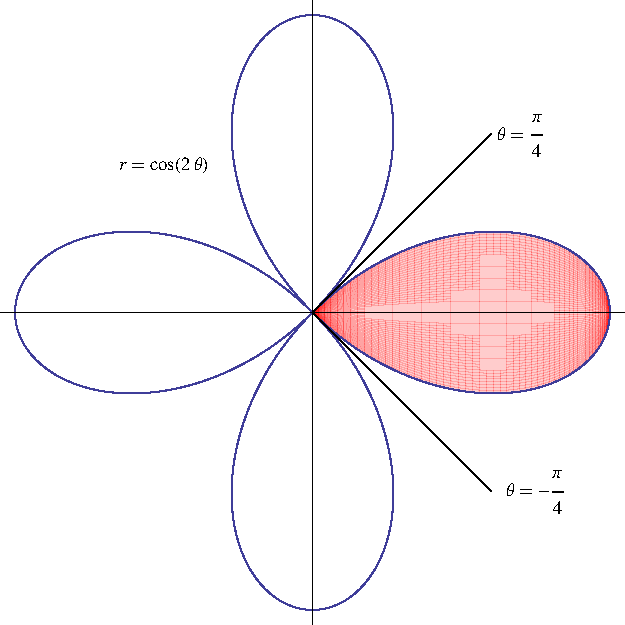
\includegraphics[height=5cm]{polar-curves/pictures/11-04-ex1a.pdf}%
}%

\uncover<2->{%
The region enclosed by the right loop is swept out by the ray that starts with $\theta = -\pi /4$ and goes to $\theta = \pi /4$.
}%
\column{.5\textwidth}
\begin{eqnarray*}
\uncover<3->{%
A%
}%
& \uncover<3->{ = } &%
\uncover<3->{%
\int_{-\pi /4}^{\pi /4}\frac{1}{2}\alert<handout:0| 4>{r^2}\diff \theta%
}\\%
& \uncover<4->{ = } &%
\uncover<4->{%
\alert<handout:0| 5>{\frac{1}{2}} \int_{\alert<handout:0| 5>{-\pi /4}}^{\alert<handout:0| 5>{\pi /4}}\alert<handout:0| 4>{\cos^22\theta} \diff \theta%
}\\%
& \uncover<5->{ = } &%
\uncover<5->{%
\int_{\alert<handout:0| 5>{0}}^{\alert<handout:0| 5>{\pi /4}}\alert<handout:0| 6>{\cos^22\theta} \diff \theta%
}\\%
& \uncover<6->{ = } &%
\uncover<6->{%
\int_{0}^{\pi /4}\alert<handout:0| 6>{\frac{1}{2}(1+\cos 4\theta )}\diff \theta%
}\\%
& \uncover<7->{ = } &%
\uncover<7->{%
\frac{1}{2}\left[ \theta + \frac{1}{4}\sin 4\theta\right]_0^{\pi /4}%
}\\%
& \uncover<8->{ = } &%
\uncover<8->{%
\frac{\pi}{8}%
}%
\end{eqnarray*}
\end{columns}
\end{example}
\end{frame}
% end module polar-area-ex1
